% !TEX program = xelatex

%%%%%%%%%%%%%%%%%%%%%%%%%%%%%%%%%%%%%%%%%%%%%%%%%%%%%%%%%%%%%%%%%%%%%%
% Source: Dave Richeson (divisbyzero.com), Dickinson College
% Version francaise par Vincent Pantaloni, prof.pantaloni.free.fr
% Traduction, correction et adaptation à la typographie française.
% 
% Une anti-seche en deux pages pour une intro rapide ou un aide mémoire des différentes fonctions. A imprimer en recto verso par exemple.
%
% Feel free to distribute this example, but please keep the referral
% to divisbyzero.com
% 
%%%%%%%%%%%%%%%%%%%%%%%%%%%%%%%%%%%%%%%%%%%%%%%%%%%%%%%%%%%%%%%%%%%%%%
%
%%%%%%%%%%%%%%%%%%%%%%%%%%%%%%%%%%%%%%%%%%%%%%%%%%%%%%%%%%%%%%%%%%%%%%

\documentclass[a4paper,11pt,landscape]{article}
\usepackage{fontspec}
\usepackage[T1]{fontenc}
\usepackage[frenchb]{babel} 
\usepackage{amssymb,amsmath,amsthm,amsfonts}
\usepackage{multicol,multirow}
\usepackage{calc}
\usepackage{ifthen}
\usepackage[landscape]{geometry}
\usepackage[colorlinks=true,citecolor=blue,linkcolor=blue]{hyperref}
\usepackage{newtxtext,newtxmath,graphicx}

\ifthenelse{\lengthtest { \paperwidth = 11in}}
    { \geometry{top=.5in,left=.5in,right=.5in,bottom=.5in} }
	{\ifthenelse{ \lengthtest{ \paperwidth = 297mm}}
		{\geometry{top=1cm,left=1cm,right=1cm,bottom=1cm} }
		{\geometry{top=1cm,left=1cm,right=1cm,bottom=1cm} }
	}
\pagestyle{empty}
\makeatletter
\renewcommand{\section}{\@startsection{section}{1}{0mm}%
                                {-1ex plus -.5ex minus -.2ex}%
                                {0.5ex plus .2ex}%x
                                {\normalfont\large\bfseries}}
\renewcommand{\subsection}{\@startsection{subsection}{2}{0mm}%
                                {-1explus -.5ex minus -.2ex}%
                                {0.5ex plus .2ex}%
                                {\normalfont\normalsize\bfseries}}
\renewcommand{\subsubsection}{\@startsection{subsubsection}{3}{0mm}%
                                {-1ex plus -.5ex minus -.2ex}%
                                {1ex plus .2ex}%
                                {\normalfont\small\bfseries}}
\makeatother
\setcounter{secnumdepth}{0}
\setlength{\parindent}{0pt}
\setlength{\parskip}{0pt plus 0.5ex}
% -----------------------------------------------------------------------

\begin{document}

\raggedright
\footnotesize

\begin{center}
     \Large{\textbf{Game Theory Cheatsheet}} \\
\end{center}
\begin{multicols*}{3}
\setlength{\premulticols}{1pt}
\setlength{\postmulticols}{1pt}
\setlength{\multicolsep}{1pt}
\setlength{\columnsep}{2pt}
\section{Static games of complete information}

\textbf{Normal form.} A NF representation is $n$ players' strategy spaces $S_1,\ldots,S_n$, and their payoff functions $u_1,\ldots,u_n: S_1\times \ldots\times S_n\to \mathbb{R}$.

\textbf{$s_i'$ strictly dominated by $s_i''$.} $\forall s_{-i}\in S_{-i}[u_i(s_i',s_{-i})<u_i(s_i'',s_{-i})]$.

\textbf{Best response.} Best response for player $i$ to other players' strategy combination $s_{-i}$ is $R_i(s_{-i})=\{s_i\in S_i:s_i\text{ maximizes }u_i(s_i,s_{-i})\}$.

\textbf{Nash equilibrium.} Strategies $(s_1^*,\ldots,s_n^*)$ are a NE if $s_i^*\in R_i(s_{-i}^*)$ for all $i$. Let $G(R_i):=\{(s_i,s_{-i}):s_i\in R_i(s_{-i}),s_{-i}\in S_{-i}\}$, then it's equivalent to $(s_1^*,\ldots,s_n^*)\in \cap_{i=1}^nG(R_i)$, equivalent to $s_i^*\in R_i(s_{-i}^*)$ for all $i$. Any $s_i^*$ in a NE cannot be eliminated in IESDS. If IESDS only returns one strategy combination, it is the unique NE.

\textbf{Cournot Model of Duopoly.} Companies choose quantities $q_1,q_2$ and sell at price $P(q_1,q_2)=(a-q_1-q_2)^+$ for $a>c$ with payoff $\pi_i=P(q_1,q_2)q_i-cq_i$. Best response is $R_i(q_j)=(a-q_j-c)/2$ if $q_j\leq a-c$ else $0$. The unique NE is $q_1^*=q_2^*=(a-c)/3$.

\textbf{Bertrand Model of Duopoly.} Two companies choose prices $p_1,p_2$ and the quantity is given by $q_i(p_i,p_j)=a-p_i+bp_j$ for some $b>0$. Profit for $i$ is $\pi_i=(a-p_i+bp_j)(p_i-c)$. $R_i(p_j)=(a+bp_j+c)/2$ and NE is $p_1^*=(a+c)/(2-b),p_2^*=(a+c)/(2-b)$. For homogeneous products, $q_i$ is defined to be $a-p_i$ if $p_i<p_j$, $0$ if $p_i>p_j$ and $(a-p_i)/2$ if $p_i=p_j$. Firm $i$'s payoff is $\pi_i=(p_i-c)q_i(p_i,p_j)$ for some $c<a$. Then $R_i(p_j)$ is $(a+c)/2$ if $p_j>(a+c)/2$, and is $[c,a]$ if $p_j=c$. The only NE is $(c,c)$ with zero net profit.

\textbf{Mixed strategy.} Let $S_i=\{s_{i1},s_{i2},\ldots,s_{iK}\}$. A mixed strategy for player $i$ is $p_i=(p_{i1},\ldots,p_{iK})$ where each $p_{ij}\geq0$ and they sum up to 1. Player $i$'s expected payoff for $(p_1,\ldots,p_n)$ is $v_i(p_1,\ldots,p_n)=\sum_{i_1=1}^{|S_1|}\ldots\sum_{i_n=1}^{|S_n|}p_{1i_1}\ldots p_{ni_n}u_i(s_{1i_1}, s_{2i_2},\ldots,s_{ni_n})$. For two-player game, mixed strategies $(p_1^*,p_2^*)$ is NE if for all possible $i$, $v_i(p_i^*,p_j^*)\geq v_i(p_i,p_j^*)$ for all possible probability distribution $p_i$ on $S_i$. If a (pure) strategy is eliminated by IESDS, then it must be played with zero probability in a NE.

\textbf{Nash's Theorem.} If $n<\infty$, $|S_i|<\infty$ for all $i$, then exists a MSNE.

\section{Dynamic games of complete information}

\textbf{Perfect information.} Player about to move knows full game history.

\textbf{Complete information.} All payoff functions are known by all players.
 
\textbf{Backwards induction outcome.} In a two player two stage game with perfect info (P1 chooses action, P2 then observes and chooses action), $(a_1^*,a_2^*=R_2(a_1^*))$ is a BI outcome, where $R_2(a_1)$ is P2's best response to P1's $a_1$, $a_1^*$ maximizes $u_1(a_1,R_2(a_1))$, maybe not $u_1(a_1,a_2^*)$.

\textbf{Stackelberg Model of Duopoly.} Same as Cournot, but firm 2 observes $q_1$ then decides. $R_2(q_1)=(a-q_1-c)/2$ if $q_1<a-c$ and 0 if $q_1\geq a-c$. $q_1^*=(a-c)/2$ maximizes $\pi_1(q_1,R_2(q_1))$.

\textbf{Subgame-perfect outcome} Two-stage game of complete but imperfect info, i.e., P1 P2 simultaneously choose actions, P3 P4 observe their actions $(a_1,a_2)$ and simultaneously choose actions. Given any $(a_1,a_2)$, P3 and P4 can find a NE $(a_3(a_1,a_2),a_4(a_1,a_2))$ in stage 2. Then P1 and P2 play a simultaneous-move game with payoffs $u_i(a_1,a_2,a_3(a_1,a_2),a_4(a_1,a_2))$. If $(a_1^*,a_2^*)$ is the NE to first stage, then $(a_1^*,a_2^*,a_3(a_1^*,a_2^*),a_4(a_1^*,a_2^*))$ is the subgame-perfect outcome.

\textbf{Tariff game.} Two countries, each has a government and a company. First G1 G2 simultaneously choose tariff rates $t_1,t_2$, then F1 F2 observe $t_1,t_2$ and simultaneously choose $(h_1,e_1),(h_2,e_2)$. Payoff to firm $i$ is $\pi_i=[a-(h_i+e_j)]h_i+[a-(h_j+e_i)]e_i-c(h_i+e_i)-t_je_i$. Payoff to Gi is $(h_i+e_j)^2/2+\pi_i+t_ie_j$. Given any pair $t_1,t_2$, stage 2 NE is $h_i^*=(a-c+t_i)/3$, $e_i^*=(a-c-2t_j)/3$. Given this, the first stage NE is $t_1^*=t_2^*=(a-c)/3$.

\textbf{Information set} for a player is a set of this player's decision nodes s.t. when reached, the player does not know which node in the set has been reached. A game with non-singleton info sets has imperfect info.

\textbf{Strategy} for a player specifies the action to take at every information set of this player. It's a function mapping each info set to an action. Let $s=(s_1,\ldots,s_n)$ be a combination of strategies of $n$ players, it yields a unique action sequence $(a_1(s),\ldots,a_m(s))$ and the payoff is defined as $\tilde{u}(s)=u(a_1(s),\ldots,a_m(s))$.

\textbf{Nash equilibrium.} The NF of a dynamic game specifies payoffs for each combination of \textit{strategies}. One can obtain a NE of the dynamic game from NF. In 2-stage game with complete and perfect info (P1 chooses then P2 observes and chooses), $(a_1^*,R_2(\cdot))$ is a NE, possibly among many others, where $a_1^*$ maximizes $u_1(a_1,R_2(a_1))$ (just like in BI). In the 2-stage game of complete but imperfect info (P1 P2 simultaneously choose, then P3 P4 observe and simultaneously choose), $(a_1^*,a_2^*,a_3(\cdot,\cdot),a_4(\cdot,\cdot))$ is a NE.

\textbf{Subgame} is a tree in EF rooted at a non-root singleton info set which does not cut any info set. A \textbf{subgame-perfect nash equilibrium} is a NE where the strategies constitute a NE in every subgame. Any finite dynamic game of complete info has a mix strategy SPNE.

\textbf{Sequential bargaining.} P1 and P2 split one dollar. $x$ dollar at time $t$ is worth $\delta^{t-k}x$ dollar at time $k$ where $\delta\in(0,1)$. Time starts at 1 (present time). Period 1: P1 proposes $(s_1(1),s_2(1))$. P2 accepts or continues. Period 2: P2 proposes $(s_1(2),s_2(2))$. P1 accepts or continues. If no agreement, in period 3, P1 P2 receives pre-defined $(\bar{s}_1,\bar s_2)$ where $\bar s_1,\bar s_2\geq0$ and $\bar s_1+\bar s_2\leq 1$. Final payoff  is $\pi_i=\delta^{t-1}s_i(t)$ (at present value) if ended in period $t$. \textbf{Lemma:} if it is known that P1 and P2 receive $(u_1,u_2)$ in period $t+1$, then in period $t$, Pi's best strategy is to offer $s_j(t)=\delta u_j$ to player $j$ who will accept. Therefore, the three-stage game has BI outcome $((1-\delta(1-\delta\bar s_1), \delta(1-\delta\bar s_1)), \text{accept})$.

\textbf{Infinite-horizon bargaining.} Continues sequential bargaining until someone accepts an offer. Let $\bar u_1,\bar u_2$ be the optimal payoffs in the BI outcome of $G$. In the third period, if not accept the offer, $G$ will be played again, with optimal payoffs $\bar u_1,\bar u_2$ settlement in period 3, then the optimal payoff for P1 is $1-\delta(1-\delta \bar u_1)$, which is identical to $\bar u_1$. Solving this, $\bar u_1=1/(1+\delta)$, $\bar u_2=\delta/(1+\delta)$.

\textbf{Infinitely repeated games.} In $t$-th stage, P1 and P2 observe actions in the preceding stages, play stage game $G$, receiving payoffs $\pi_{1,t},\pi_{2,t}$. Final payoff is $(\sum_{t=1}^\infty\delta^{t-1}\pi_{1,t}, \sum_{t=1}^\infty\delta^{t-1}\pi_{2,t})$. $A_{it}$ is the acion space for player $i$ in stage $t$, $A_t=A_{1t}\times A_{2t}$. A strategy of player $i$ is a function $a_{it}:A_1\times\ldots\times A_{t-1}\to A_{it}$ as a map from action history of the first $t-1$ stages to an action. Stage game, where $0<x<y<z$:
\vspace*{-8pt}
\begin{center}
    \begin{tabular}{lll}
                               & $L_2$                      & $R_2$                      \\ \cline{2-3} 
    \multicolumn{1}{l|}{$L_1$} & \multicolumn{1}{l|}{$x,x$} & \multicolumn{1}{l|}{$z,0$} \\ \cline{2-3} 
    \multicolumn{1}{l|}{$R_1$} & \multicolumn{1}{l|}{$0,z$} & \multicolumn{1}{l|}{$y,y$} \\ \cline{2-3} 
    \end{tabular}
\end{center}

\textbf{Non-cooperative strategy} ($NC_i$) is a strategy where a player plays a strategy from a NE in every stage, i.e., $L_i$. A \textbf{trigger strategy} ($T_i$) is to play $R_i$ if all preceding stages have been $(R_1,R_2)$, else play $L_i$. First, (NC1,NC2) is a NE. (T1,T2) is NE if and only if $y+\delta y+\delta^2y+\ldots\geq z+\delta x+\delta^2x+\ldots$, i.e., $\delta\geq(z-y)/(z-x)$. (T1,T2) is a SPNE as any subgame strategy is either (NC1,NC2) or (T1,T2).

\textbf{Cournot duopolists' collusion.} Similarly, the NE for single stage Cournot is both choose $q_c=(a-c)/3$, receiving $p_c=(a-c)^2/9$. If there's only one firm, the optimal is to produce $q_m=(a-c)/2$ with profit $p_m=(a-c)^2/4$. A cooperative strategy would be to produce $q_m/2$ each with profit $p_m/2$. If the other firm produces $q_m/2$, the best response is $3(a-c)/8$ with profit $p_d=9(a-c)^2/64$. (T1,T2) is NE iff $p_m/2+\delta p_m/2+\delta^2 p_m/2+\ldots\geq p_d + \delta p_c+\delta^2p_c+\ldots$, i.e., $\delta\geq9/17$.

\section{Static games of incomplete information}

\textbf{Bayesian games} are games with incomplete info where at least one player is uncertain about another player's payoff function. NF of a $n$-player static Bayesian game (SBG) specifies action spaces $A_1,\ldots,A_n$, type spaces $T_1,\ldots,T_n$, beliefs $P_1,\ldots,P_n$ and payoff functions $u_1,\ldots,u_n$. $t_i\in T_i$ is known only by player $i$. Payoff function depends on type $u_i(a_1,\ldots,a_n;t_i)$. Player $i$'s belief $P_i(t_{-i}|t_i)$ is the probability of any $t_{-i}$ conditioned its own type $t_i$.

\textbf{Beliefs in SBG.} If types $t=(t_1,\ldots,t_n)$ is drawn by nature from prior prob. distr. $P(t)$, then $P_i(t_{-i}|t_i)=P(t_{-i},t_i)/(\sum_{t_{-i}'\in T_{-i}}P(t_{-i}',t_i))$.

\textbf{Strategies in SBG.} A strategy for player $i$ is a func $s_i:T_i\to A_i$, maps each own type to action. Strategy space is the set of all such functions.

\textbf{Bayesian NE.} In SBG, strategies $s^*=(s_1^*,\ldots,s_n^*)$ are pure BNE if for all $i$, for all $t_i\in T_i$, $s_i^*(t_i)$ maximizes $E_{t_{-i}}u_i(a_i,s_{-i}^*(t_{-i});t_i)$, i.e., $\sum_{t_{-i}\in T_{-i}} P_i(t_{-i}|t_i)u_i(a_i,s_{-i}^*(t_{-i});t_i)$. Mixed BNE exists if finite $A_i$. 

\textbf{Finding BNE.} For player $i$, for each type $t_i$, list payoffs (expected, if other player has more than one types) of all actions given the other player's strategies, find the best response to every strategy of the other player. The interaction of all best response correspondence is BNE.

\textbf{Nature selects a game.} Define a SBG as $\{G,P,(T_1,\ldots,T_n)\}$. $G$ is a set of games, any $g\in G$ specifies players' action spaces $A_i$ and payoffs $u_i(a;g)$. $P$ is the distribution on $G$, i.e., how nature selects a game. $T_i$ is player $i$'s type space, it is a partition of $G$. Any type $t_i\in T_i$ is a subset of $G$. If $g$ is chosen, then the player knows its type $\sigma_i(g)$ as the set in $T_i$ that contains $g$, where $sigma_i:G\to T_i$ such that $\sigma_i(g)=t_i$ iff $g\in t_i$.

\textbf{Expected payoff.} Given strategies $s_{-i}:T_{-i}\to A_{-i}$ of other players, $u_i(a_i,s_{-i};t_i)$ is the expected payoff for player $i$ of type $t_i$ if play $a_i$ and others play $s_{-i}$, equals $1/P(t_i)\cdot\sum_{g\in t_{i}} P(g)u_i(a_i,s_{-i}(\sigma_{-i}(g));g)$.

\textbf{Finding BNE.} When it is convenient to use the ``nature selects a game" model, one uses the same procedure to find BNE as previously described, but uses game probabilities for expected payoff calculation.

\textbf{First-price sealed-bit auction.} P1 P2 have valuations $v_1,v_2$ indp and unif on $[0,1]$ as types. Bids $b_1,b_2\in[0,\infty]$ are simultaneous actions. $P_i(v_j)$ is uniform distr on $[0,1]$. Given type $v_i$, player $i$'s payoff is $u_i(b_1,b_2;v_i)=v_i-b_i$ if $b_i>b_j$, $(v_i-b_i)/2$ if $b_i=b_j$ and $0$ if $b_i<b_j$. Strategies $(b_1(\cdot),b_2(\cdot))$ is a BNE if $\forall v_i\in[0,1]$, $b_i(v_i)$ maximizes $E_{v_j} u_i(b_i,b_j(v_j);v_i)=(v_i-b_i)\Pr[b_i>b_j(v_j)]\allowbreak+\allowbreak(v_i-b_i)/2\allowbreak\Pr[b_i=b_j(v_j)]$. Linear strategies $b_i(v_i)=a_i+c_iv_i$ where $0\leq a_i<1,c_i>0$. The only linear BNE is $(v_1/2,v_2/2)$.


\section{Dynamic games of incomplete information}

\textbf{Limitation of SPNE.} In dynamic games, even subgame-perfect Nash equilibrium can have noncredible threats as it does not guarantee optimal action at every information set (but at every subgame).

A \textbf{perfect Bayesian equilibrium} consists of strategies and beliefs such that: (i) \textbf{consistency}: at every info set, beliefs are determined by Bayes'rule and strategies whenever possible. For a node inside an info set, the belief about this node is the probability of reaching this node conditioned on reaching this info set starting from the root of the smallest subgame containing this info set, when all players play the given strategies. If the info set cannot be reached under given strategies, then any belief is consistent. (ii) \textbf{sequential rationality}: at each info set, action of the players about to move (and subsequent actions of the player) must be optimal given the belief (maximizing the expected payoff based on beliefs), when others play by the given strategies.

\textbf{Finding PBE.} One can verify every strategy for PBE: find consistent beliefs and check the strategies are indeed optimal given these beliefs. Strategies in any perfect Bayesian equilibrium is a Nash equilibrium. So one only needs to check NEs.

\textbf{Signaling.} Nature draws sender type $t_i\in T=\{t_1,\ldots,t_I\}$ according to $\Pr[t_i]$. Sender observes $t_i$ and chooses message $m_j\in M=\{m_1,\ldots,\allowbreak m_J\}$. Receiver observes $m_j$ but not $t_i$, and chooses action $a_k\in A=\{\allowbreak a_1,\ldots,a_K\}$. Payoff determined by $t_i,m_j,a_k$ (so for receiver it's expected). See figure for a signaling game with 2 types and 2 actions. Sender strategy is a map from type to message, receiver strategy is a map from message to action. For sender, \textbf{pooling} strategies send same messages for each type, while \textbf{separating} strategies send different messages for different types.

\textbf{Signaling PBE.} Receiver has belief $\mu$ on types given $m_j$. Strategies $m^*(t_i),a^*(m_j)$ and belief $\mu(t_i|m_j)$ is PBE if (i) consistency: $\mu(t_i|m_j)\allowbreak=P(t_i)/\sum_{t\in T_j} P(t)$ where $T_j$ is the set of types s.t. $m^*(t_i)=m_j$. If $T_j=\emptyset$, any $\mu$ is consistent. (ii) sequential rationality: for each $m_j$, receiver's action $a^*(m_j)$ maximize $\sum_{t_i\in T}\mu(t_i|m_j)U_R(t_i,m_j,a_k)$, and for each $t_i\in T$, sender's message $m^*(t_i)$ maximize $U_s(t_i,m_j,a^*(m_j))$.
For a PBE of signaling game, if sender strategy is pooling/separating, we call the PBE pooling/separating.

\textbf{Finding PBE in signaling games.} One can check every possible sender strategy. Given sender strategy, one can calculate the consistent belief. With belief, one can determine receiver strategy and at last whether the sender strategy is optimal in the first place. Alternatively, one can also give NF of the game, where for each strategy $m(t_i), a(m_j)$, the payoff is expected over how nature selects the type. NF gives a NE of the game and one can verify the NE to find PBE.

\textbf{Signaling games with continuous receiver actions.} Nature selects worker's ability $\eta\in\{\eta_H,\eta_L\}$. Worker knows $\eta$, chooses education $e\in\{e_c,e_s\}$. Firm observes $e$ and decides wage $w\in[0,\infty)$.

\begin{center}
    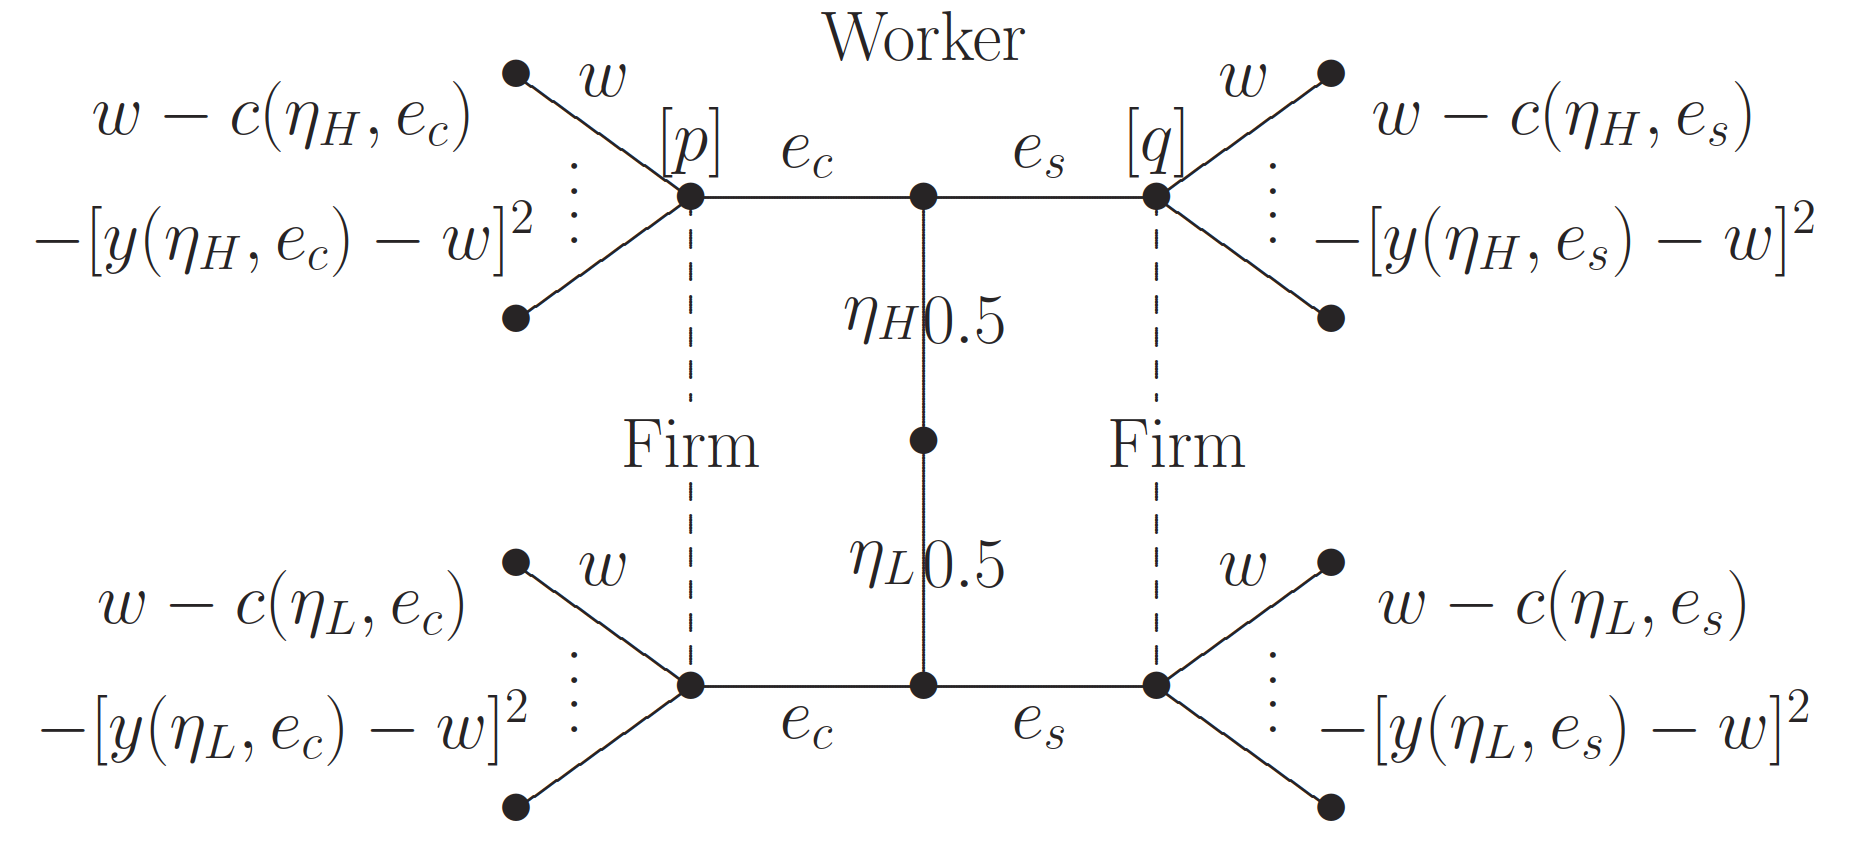
\includegraphics[width=\linewidth]{job_market_signaling.png}
\end{center}

If $c(\eta,e)=c_1(\eta)+c_2(\eta)$, then any PBE must be pooling. The idea is that if it is optimal for worker to choose $e_c$ in one type, it must be optimal to also choose $e_c$ in the other type. Therefore, one just checks the pooling strategies. If the worker pools on $e_i$, then belief probability of $\eta_L$, $r$, is determined. Firm maximize $-r[y(\eta_H,e_i)-w]^2-(1-r)\allowbreak[y(\eta_L,e_i)-w]^2$ by $w^*(e_i,r)=ry(\eta_H,e_i)+(1-r)y(\eta_L,e_i)$.

If worker do $(e_c,e_c)$, then $p=1/2$ and $q$ can be any value. $(e_c,e_c)$ is indeed optimal under $\eta$ iff $y(\eta_H,e_c)/2+y(\eta_L,e_c)-c1(\eta)-c_2(e_c)\allowbreak\geq qy(\eta_H,e_s)+(1-q)y(\eta_L,e_s)-c_1(\eta)-c_2(e_s)$. Let $B(\eta,e)=y(\eta,e)-c_2(e)$. Then $(e_c,e_c)$ is optimal iff $B(\eta_H,e_c)/2+B(\eta_L,e_c)/2\geq qB(\eta_H,e_s)+(1-q)B(\eta_L,e_s)$, since $B$ increases with $\eta$, this is true for all $q\leq\bar q$ for some $\bar q\in[0,1]$. Hence, $\{(e_c,e_c),(w^*(e_c,p),w^*(e_s,q)),p=1/2,q\in[0,\bar q]\}$ is a PBE. Similar for $(e_s,e_s)$.


\end{multicols*}

\end{document}

% \href{http://amath.colorado.edu/documentation/LaTeX/Symbols.pdf}{\LaTeX\ Mathematical Symbols}\\
% \href{ftp://tug.ctan.org/pub/tex-archive/info/symbols/comprehensive/symbols-letter.pdf}{The Comprehensive \LaTeX\ Symbol List}\\ 
% \href{http://mirrors.med.harvard.edu/ctan/info/lshort/english/lshort.pdf}{The Not So Short Introduction to \LaTeX\ 2$\varepsilon$}\\
% \href{http://www.tug.org/}{TUG: The \TeX\ Users Group}\\
% \href{http://www.ctan.org/}{CTAN: The Comprehensive \TeX\ Archive Network}\\
% \LaTeX\ for the Mac: \href{http://www.tug.org/mactex/}{Mac\TeX}\\
% \LaTeX\ for the PC: \href{http://www.texniccenter.org/}{{\TeX}nicCenter} and \href{http://miktex.org/}{MiK\TeX}\\
% \LaTeX\ online: \href{http://www.writelatex.com/}{WriteLaTeX}.